% Please write one sentence per line! (easier for version control)

\documentclass[10pt, a4paper]{article}
\usepackage{lrec2006}
\usepackage{graphicx}
\usepackage{todonotes}
\usepackage{linguex}
\usepackage{amssymb}

\title{Towards text mining in environmental science:\\
extraction of quantitative variables and their relations}

\name{Author1, Author2, Author3}

\address{ Affiliation1, Affiliation2, Affiliation3 \\
               Address1, Address2, Address3 \\
               author1@xxx.yy, author2@zzz.edu, author3@hhh.com\\}


\abstract{
This paper addresses text mining in the cross-disciplinary domain of environmental science and climate science.
It is motivated by the desire for literature-based knowledge discovery from scientific publications.
The particular goal is to automatically extract relations between quantitative variables from raw text.
This results in rules of the form ``If variable X increases, than variable Y decreases''.    
As a first step in this direction, an annotion scheme is proposed to capture the events of interest -- those of change, cause, correlation and feedback -- and the entities involved in them -- quantitative variables.
Its purpose is to serve as an intermediary step in the process of rule extraction.
It is shown that the desired rules can indeed be automatically extracted from annotated text.
A number of open challenges are discussed, including automatic annotation, normalization of variables, reasoning with rules in combination with domain knowledge and the need for meta-knowledge regarding context of use.
\\ \newline 
\Keywords{Text Mining, Literature-based Knowledge Discovery, Environmental Science, Climate Science, Corpus Annotation, Relation Extraction, Event Extraction}}

\newcommand{\tag}[1]{\textsc{#1}}

% Define your own todo notes here, like 
% \newcommand{\XX}[1]{\todo[inline,author=XX,color=YY]{#1}}
\newcommand{\EM}[1]{\todo[inline,author=EM,color=yellow]{#1}}
\newcommand{\EA}[1]{\todo[inline,author=EA,color=green]{#1}}



\begin{document}

\maketitleabstract

%=============================================================================
\section{Introduction}
%=============================================================================

\todo[inline]{Argue that text mining in environmental sciences:
has not been really pursued so far;
is different from text mining in biomedicine}

\todo[inline]{Applications: search, QA, etc}.

The scientific literature is growing so rapidly that researchers have been forced to become increasingly specialized to keep up with the state-of-the-art. 
This specialization can lead to the fragmentation of science, as researchers from different (sub-)disciplines rarely have time to read each other's papers. 
\newcite{Swanson1986Undiscovered} claimed that this fragmentation of science gives rise to \emph{undiscovered public knowledge}, i.e. still unmade inferences that can be made based on publicly available knowledge. As an example, he hypothesized that fish oils can cure Raynaud's disease by combining two publicly available statements: 1) Fish oils reduce blood viscosity, 2) patients with Raynaud's disease tend to exhibit high blood viscosity \cite{Swanson1986Fishoil}. 
This method of making hypothesis inferences of the form $A \to C$ based on publicly available statements $A \to B$ and $B \to C$ has been termed \emph{Swanson linking}\footnote{In the Swanson linking paradigm, the operator $\to$ is not interpreted as a logical conditional, but rather as an abstract causal or correlative relation between the terms. The conclusion $A \to C$ is therefore not logically sound, but has nevertheless been showed to give empirically useful results.}. 

The discoveries of Swanson prompted a line of research into methods for computer support in the identification of undiscovered public knowledge, an area which has been labelled Literature-based discovery (LBD). 
Most LBD methods are based on Swanson linking, and use term co-occurrence frequencies to detect relations of the type $A \to B$. 
Terms are usually extracted as n-grams from the text \cite{Lindsay1999LBDLexicalStat} or taken from a controlled vocabulary or ontology \cite{Weeber2001ConceptsInLBD}.

Recently, co-occurrence based methods have come under critique for leading to too many spurious discoveries.
\newcite{Hristovski2008NLPinLBD} therefore advocate an approach based on Natural Language Processing (NLP), as such approaches are able to be more specific about the relation that holds between two terms. 
LBD efforts have traditionally been undertaken in the biomedical domain, and have therefore benefited from existing biomedical NLP tools such as SemRep\footnote{http://semrep.nlm.nih.gov/}.
Application of NLP-based LBD techniques to less resourced domains, such as the environmental sciences, would however require the development or adaptation of NLP tools to the new domain.

\todo[inline]{Related work (possibly in separate section or in Discussion section):
\cite{Hashimoto2012Excitatory}
\cite{Mihaila2013BioCause}
\cite{Zambach2010Lexical}
\cite{Vossen2008}}

The remainder of this paper is structured as follows. 
The next Section proposes a new annotation scheme to capture the events of interest -- those of change, cause, correlation and feedback -- and the entities involved in them -- quantitative variables. 
Section~\ref{sec:extraction} shows that  rules can indeed be automatically extracted from annotated text.
Section~\ref{sec:discussion} discusses a number of open challenges are discussed, including automatic annotation, normalization of variables, reasoning with rules in combination with domain knowledge and the need for meta-knowledge regarding context of use.
The last Section closes with conclusions and future work.

%=============================================================================
\section{Annotation}
%=============================================================================

\subsection{Procedure}

The data consisted of 12 abstracts (2369 words) from recent, high-quality scientific journal publications about the relation between climate and ocean changes. 
These were selected by our domain expert (author MVA) as a reasonably representative sample of the text type in the targeted area, comprissing multi-disciplinary work in marine biology, marine science, oceanography, environmental science, climate science, biogeoscience and geophysics.
Text was automatically extracted from PDF files.
Abstracts were manually extracted, tokenized and split into sentences, also allowing for manual correction of minor PDF-to-text conversion errors.

Annotation was carried out using the Brat annotation tool \cite{stenetorp2012}.
The annotion scheme described below was developed in an iterative fashion in close colaboration with our domain expert.
It is inspired by annotation efforts in the biomedical domain such as the GENIA corpus \cite{Kim2003GENIA} and the corpora used in the BioNLP shared tasks on event extraction \cite{Kim2009Overview}.
It covers a particular type of events -- those of change, cause, correlation and feedback -- and the entities involved in them -- quantitative variables.
The primary reason of annotation is not to analyse the text according to some linguistic formalism or theory, or to follow some knowledge representation formalism or ontological theory.
Instead the purpose of the annotation is rather pragmatic: to serve as an intermediary step in the process of extracting rules about the relation between quantitative variables from raw text.      
 
The annotation scheme proposed below seems a good candidate for this purpose.
However, it remains to be seem how it holds up when applied to more text.
Inter-annotator agreement has not been measured so far.
\EM{Probably better to merge this paragraph into Discussion section} 

\subsection{Annotation scheme}

The resulting annotation scheme involves one type of entity (variable), several types of events (change, increase, decrease, cause, correlate, feedback) and some basic logic structure (and/or, negation).  


\subsubsection{Variables}

A quantitative variable is an entity that can be counted or measured.
Its value can be naturally expressed by a number such as a count, a ratio, a percentage or a scalar (quantity of units).
It can be regarded as a (potential) quantitative variable in an experiment or a model. 
Not every variable in the text is labeled as such.
To save annotation time and effort, only those variables related to a change are annotated.
The  direction of change can be positive (increasing), negative (decreasing) or unspecified (either increasing or decreasing), but there must always be a clear cue in the text that the variable is involved in some change. 
Examples of changing, increasing and decreasing variables respectively:

\ex.
  \a. significant changes in [\emph{surface ocean pH}]
  \b. rise in [\emph{atmospheric CO2 levels}]
  \c. decline in [\emph{marine primary production}]

In contract, the text spans in \Next are not annotated as variables.

\ex.
  \a. *[\emph{carbon dioxide}] and [\emph{light}] are two major prerequisites of photosynthesis
  \b. *changes in [\emph{the network of global biogeochemical cycles}] 
  \c. *The concentrations of [\emph{DFe}] and [\emph{TaLFe}] were relatively high

The text spans in \Last[a] are measurable, in principle at least, but there is no textual cue in the context indicating that they are subject to change. 
The text span in \Last[b] admittedly identifies something that is changing, but it is an abstraction -- not something that can be measured and naturally expressed through a number. 
The ones in \Last[c] express a static state rather than a dynamic event.
The reason for excluding cases like these is that they do not lead to useful rules about the relation between quantitative variables.

Variables must be indicated as precisely as possible, that is,including any relevant specifications, modifications or conditions. So instead of \Next[a], \Next[b] is prefered.

\ex.
  \a. *a difference in [\emph{carbon concentration}] between the ocean surface and the deep waters
  \b. a difference in [\emph{carbon concentration between the ocean surface and the deep waters}]

The choice is motivated by the idea that, given a syntactic parse, it is usually easier to generalize a complex argument by stripping modifiers than the other way around.  

Variables are tagged with the label \tag{Variable}. It is most likely advantaguous to distinguish different subclasses of variables. Currently we are not concerned with this. 
However, we do not exclude the possibility of a more fine-grained annotation at a later stage. 


\subsubsection{Change, Increase and Decrease}

A change is an event in which the value of a quantitative variable is changing.
The direction of change can be positive (increasing), negative (decreasing) or unspecified (either increasing or decreasing), but there must always be a clear cue in the text that the variable is involved in a change.
This is referred to as the \emph{trigger} for the event.

Examples of triggers for event types of change, increase and decrease are:

\ex.
  \a. [\emph{regional changes}] in phytoplankton
  \b. [\emph{addition of}] labile dissolved organic carbon
  \c. [\emph{to slow down}] calcification in corals

Changes must apply to a variable; hence the text span in \Next does not trigger a

\ex. *marine primary production is sensitive to climate [\emph{variability and change}]

Events of increase, decrease and undirected changes are tagged as \tag{Increase}, \tag{Decrease} and \tag{Change} respectively. 
Events are related to variables through thematic roles, which specify the different participants in the event. 
Change events must always have a \tag{Theme} role that is filled by the variable that is changing.
Typical annotation examples are therefore:\footnote{We use labeled brackets to denote enitities, events or thematic roles, depending on the context of discussion.}

\exi.
  \a. [\tag{Decrease} reduced] [\tag{Theme} calcite production]
  \b. [\tag{Change} significant changes in] [\tag{Theme} surface ocean pH]

In addition, they can optionally have an \tag{Agent} role or a \tag{Co-theme} role, which will be explained in the next Section.

Change events can also function as Cause/Correlate events, as will be described in the next Section, in which case they take an AGENT or CO-THEME role as well.


\subsubsection{Cause}

Cause events involve a pair of changes where the first change causes the second change.
Since a change event involves a changing variable, as its theme, causal events thus express a causal relation between two changing variables. 
The trigger of a cause event is annotated with a \tag{Cause} tag.
Triggers are often verbs, but can also be adjectives (\emph{stimulatory}), adverbs (\emph{therefore}) or subjunctive phrases (\emph{due to}, \emph{in response to}) and other phrasal expression (\emph{has an effect on}).  

Cause events must always have two thematic roles: an \tag{Agent} identifying the cause and a \tag{Theme} identifying the effect. 
% Notice that causal relations are directional. 
% That if, if  A causes B, then it does not follow that B causes A.
Examples of cause events are:

\exi.
  \a. [\tag{Agent} rise in atmospheric CO2 levels] [\tag{Cause} \emph{causes}] [\tag{Theme} significant changes in surface ocean pH]
  \b. [\tag{Agent} Fe(III) addition in the presence of GA (FeGA)] [\tag{Cause} \emph{gave}] [\tag{Theme} higher Fe(II) concentration]
  \c. [\tag{Agent} diminished calcification] [\tag{Cause} \emph{led to}] [\tag{Theme} a reduction in the ratio of calcite precipitation to organic matter production]
% number of examples can be reduced

In many cases, a cause event and a change event share one and the same trigger, as in the following examples:

\exi.
  \a. [\tag{Agent} changes in the magnitude of total and export production] [\tag{Change} \emph{can strongly influence}] [\tag{Theme} atmospheric CO2 levels]
  \b. [\tag{Theme} calcification and net primary production] [\tag{Increase} \emph{ are significantly increased by}] [\tag{Agent} high CO2 partial pressures]
  \c. [\tag{Agent} addition of labile dissolved organic carbon] [\tag{Decrease}  \emph{reduced}] [\tag{Theme} phytoplankton biomass]

In \Last[a], \emph{can strongly influence} serves as the cue for a change event with variable \emph{atmospheric CO2 levels} as its theme. 
At the same time, it is the trigger for a cause event with agent \emph{ changes in the magnitude of total and export production} and theme \emph{atmospheric CO2 levels}.
In principle, both events can be annotated individually.  
However, in order to avoid a needlessly complex annotation, we choose to not annotate the cause event explicitly. 
Instead \emph{changes in the magnitude of total and export production} is given the role of agent in the change event. 
Presence of an agent role suffices to infer the cause event.
Two more instances of this pattern are shown in \Last[b] and \Last[c].

\EM{Describe exceptional cases of variable with implicit change}


\subsubsection{Correlate}

Correlate events involve a pair of changes where the first change correlates with the second change. 
Since a change event involves a changing variable, as its theme, correlate events thus express a correlation between two changing variables. 
That is, if one of them changes, the other changes along. 
Correlations  have two roles, \tag{Theme} and \tag{Co-theme}, both of which should be fulfilled by a change event (i.e. \tag{Increase}, \tag{Decrease} or \tag{Change}).
% or a quantitative variable (Variable)
Examples of correlate events:

\exi.
  \a. [\tag{Theme} reduced calcite production] [\tag{Correlate} \emph{ was accompanied by}] [\tag{Co-theme} an increased proportion of malformed coccoliths]
  \b. [\tag{Theme} carbon:nutrient ratio turns out to decrease] [\tag{Correlate}  \emph{with}] [\tag{Co-theme} increasing mixed-layer depth and temperature]
  \c. Here we report [\tag{Them}e reduced calcite production] [\tag{Correlate}  \emph{at}] [\tag{Co-theme} increased CO2 concentrations]
  \d. [\tag{Correlate} \emph{When}] [Co-theme bacterial growth rate was limited by mineral nutrients], [Theme extra organic carbon accumulated in the system]
%  \e. [\tag{Theme} regional changes in phytoplankton] [\tag{Correlate} coincide with] [\tag{Co-theme} observed changes in kril]

Notice that correlation can be triggered by a verb \Last[a], a preposition \Last[b-c] or an adverb/conjunction \Last[d].

Statistically speaking, correlation is not a directional relation, in contrast to causation. That is, if a change in variable A is correlated with a change in variable B, then it follows that a change in variable B is correlated with a change in variable A. However, in discourse there is often a distinction between a variable of interest (the dependent variable) and related variable (the independent variable). 
Thus even though strictly speaking there is no causal relation between the two variables, the text usually takes a particular perspective, suggesting one is more central than the other. 
By convention, the central variable is tagged as \tag{Theme}, whereas the other one is tagged as \tag{Co-theme}. 
The rule of thumb is that the co-theme is syntactically the argument of a preposition (e.g. \emph{with, at, under}) or an adverb/conjunction (e.g. \emph{when}).  

Occasionally correlations can hold between a change event and a variable, or even between two variables, rather than between to change events.
In these exceptional cases, we assume the variable is interpreted as changing (i.e. as being part of an implicit change event), because it is involved in a correlate event.
Two examples of this exceptional pattern are: 

\exi.
  \a. [\tag{Increase} Concentrations of DFe increased slightly] [\tag{Correlate} with]  [\tag{Variable} depth in the water column]
  \b. [\tag{Variable} growth rates in the high-CO2-grown cells] [\tag{Correlate} were related to] [\tag{Variable} light level]


In \Last[a], the role of co-theme is not taken by a change event, but by the variable \emph{depth in the water column}.
It is thus assumed that the depth in the water column is a changing variable in the correlation described.
Similarly, \Last[b] has both roles of the correlate event taken up by variables, which are therefore interpreted as subject to change.

\EM{Should we allow the same for \tag{Cause}? Check data} 
\EA{Perhaps we can move this discussion, together with the discussion of inherently changing variables (Ocean Acidification, etc), to a new sub-chapter about variables that are interpreted as changing without an explicit change?}

\subsubsection{Feedback}

Feedback loops are an important concept in climate science. An example is that of the relation between rising temperature and methane release: a rise in temperature causes more permafrost to melt, which causes more release of methane in the atmosphere (a ``green house'' gas), which causes further rising of the temperature, and so on.
However, explicit mentioning of feedback events in the text appears to be rare compared with the frequent occurrence of change events, so our proposal for annotation of feedbacks is currently based on only a couple of instances.
Feedback events hold between two variables, filling the roles of \tag{Theme} and \tag{Co-theme}, as exemplified below: 

\exi. our model suggests the existence of [\tag{+Feedback} a positive feedback between] [\tag{Theme} temperature] and [\tag{Co-theme} atmospheric CO2 content]

Analogously to change events, feedback events can positive (self-sustaining, self-enhancing), negative (self-stabilizing, self-diminishing) or of unspecified polarity. 

\EM{Consider including positive, negative and unspecified correlation too. Looks better than having an 'inverse' attribute for negetaive correlation.}


\subsubsection{Referring expressions}

Referring expressions such as anaphoric expressions (e.g. \emph{it}, \emph{this}) and underspecified definite descriptions (e.g. \emph{the process}) are annotated only in so far as they play a thematic role in an event of interest. Consider the following narrative:

\exi. 
  \a.[s1:] Future shoaling of upper-mixed-layer depths will expose phytoplankton to [\tag{Increase} increased] [\tag{Theme} mean light intensities].
  \b.[s2:] [\tag{RefExp/Agent} \emph{This}] [\tag{Cause} may cause] [\tag{Decrease} a widespread decline in] [\tag{Theme} marine primary production]

The first sentence contains an \tag{Increase} event, which is referred to in the second sentence by means of the referring expression \emph{This}, establishing it as the cause for the\tag{Decrease} event.
The referring expressions must therefore be resolved in order to arrive at the rule an increase in mean light intensities causes a decrease in marine primary production.
In order to achieve this, such referring expressions are tagged as \tag{RefExp} and connected with their antecedent by means of a \tag{Coref} relation. 
  

\subsubsection{Combinations}

Variables or events can be combined through conjunction or disjunction.
Such combinations are labeled as \tag{And} or \tag{Or}, where their constituents fill the role of \tag{Part}.
In \Next[a], for example, the combination \tag{And} serves as the theme of the \tag{Increase} event.
Likewise, two increasing events are combined to serve as the theme in a causal event.

\exi.
  \a. [\tag{Increase} increasing [\tag{Part:Variable} mixed-layer depth] [\tag{Theme:And} and] [\tag{Part:Variable} temperature]  
  \b. [\tag{Cause} gave] [\tag{Part:Increase} higher ] Fe(II) concentration [\tag{Theme:And} and] [\tag{Part:Increase} higher] growth rate of phytoplankton

The alternative option in \Last[a] is to tag the whole combined phrase as a single variable.
We chose not do so because coordination is notoriously hard problem for syntactic parsers and any help from the annotation in resolving ambiguity should be exploited.
Notice also that a similar option is not availabe in \Last[b], as considering the whole combination as a single change event would result in loss of substantial information.


\subsubsection{Negation}

Events can carry a negation attribute to account for examples such as:

\exi.
  \a. TaLFe [\tag{Correlate+Neg} did \emph{not} show any consistent trend with] depth 
  \b. [\tag{Change+Neg} \emph{No} differences] in cellular organic carbon:nitrogen ratios were observed

Triggers for negation are currently not explicitly annotated.


%=============================================================================
\section{Rule extraction}
%=============================================================================
\label{sec:extraction}

See Figure~\ref{fig:ex1}. 
See Figure~\ref{fig:ex2}. 
See Figure~\ref{fig:ex3}.

\setlength{\fboxsep}{10pt}

\begin{figure*}
\begin{center}
\framebox[\textwidth]{
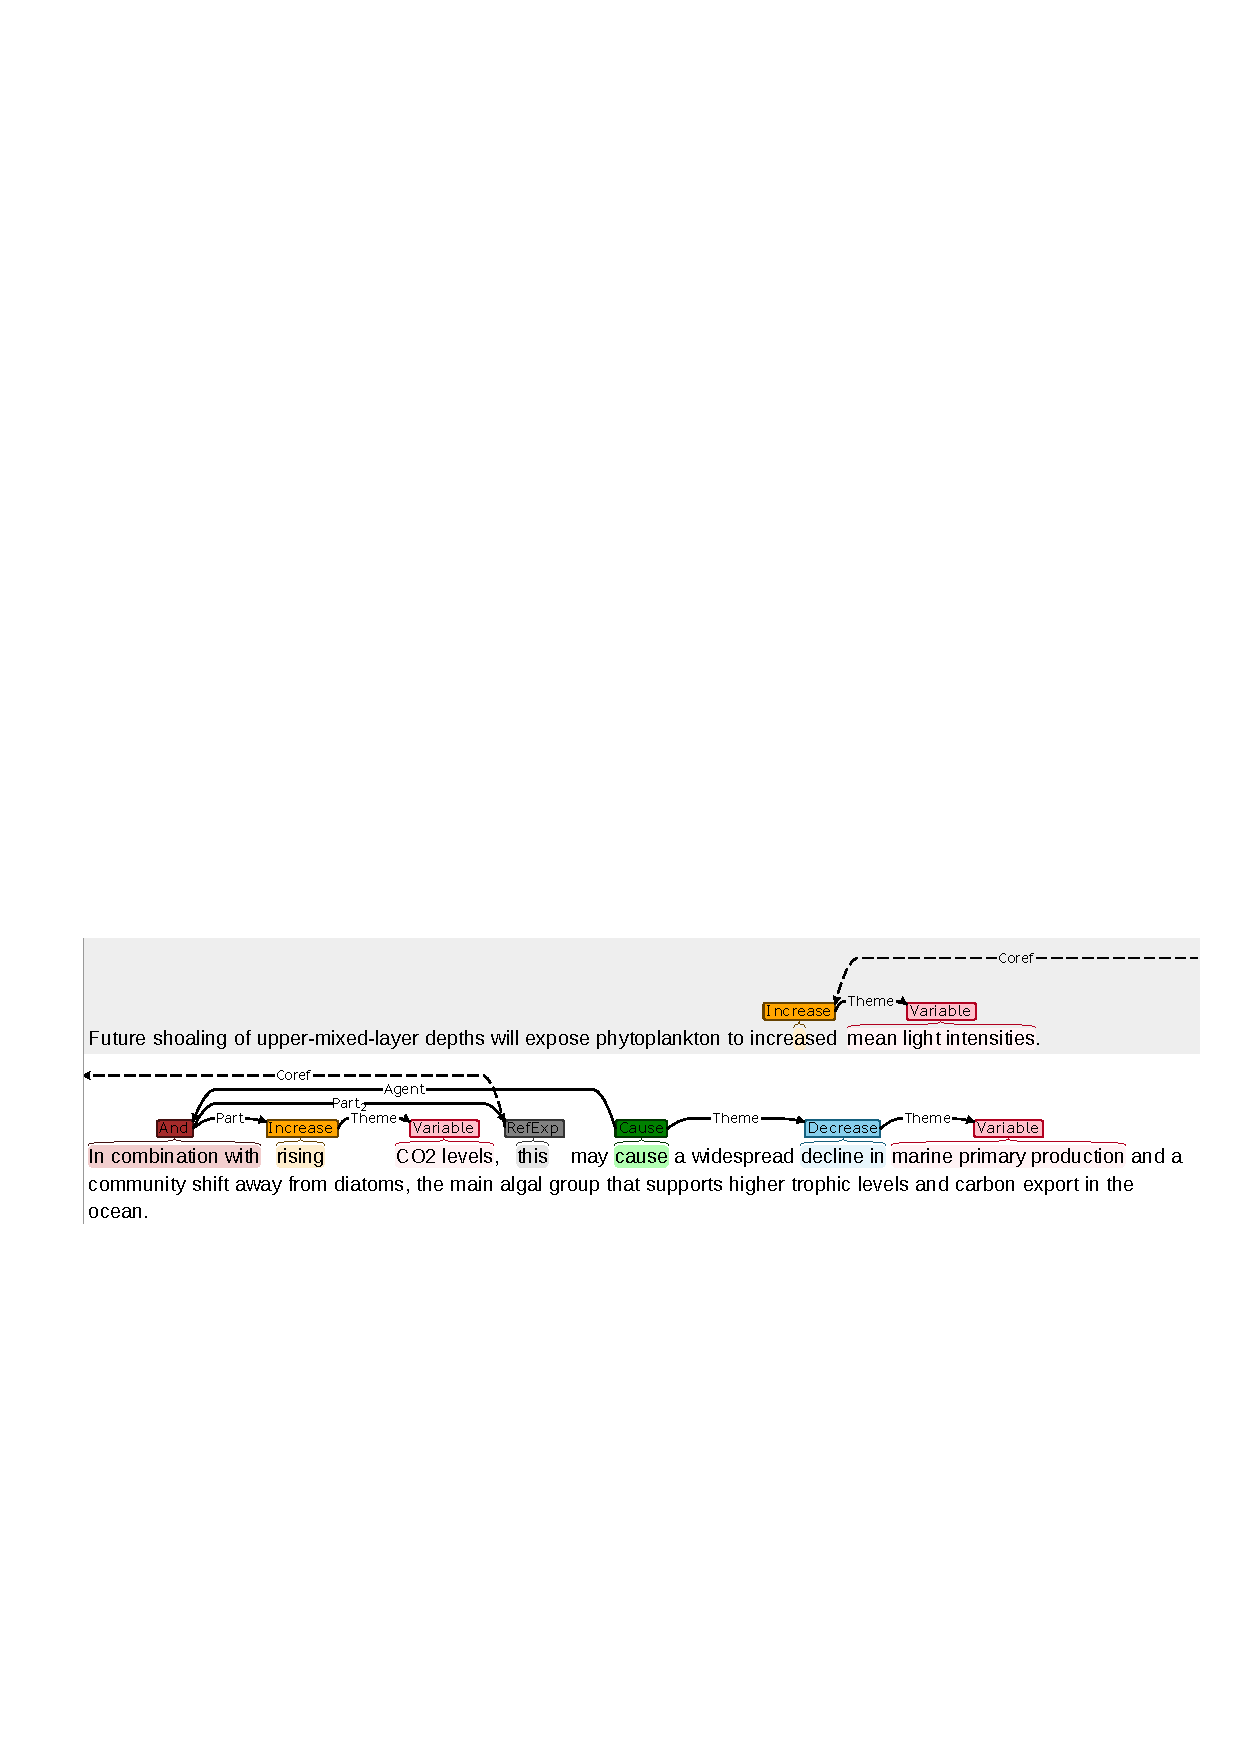
\includegraphics[scale=0.9]{ex1.pdf}}
\framebox[\textwidth]{[ $\uparrow$ mean light intensities $\wedge$ $\uparrow$ CO2 levels ]~~~ $\Longrightarrow$~~~$\downarrow$ marine primary production}
 \caption{Example of a causal rule extracted from a pair of annotated sentences}
\end{center}
\label{fig:ex1}
\end{figure*}


\begin{figure*}
\begin{center}
\framebox[\textwidth]{
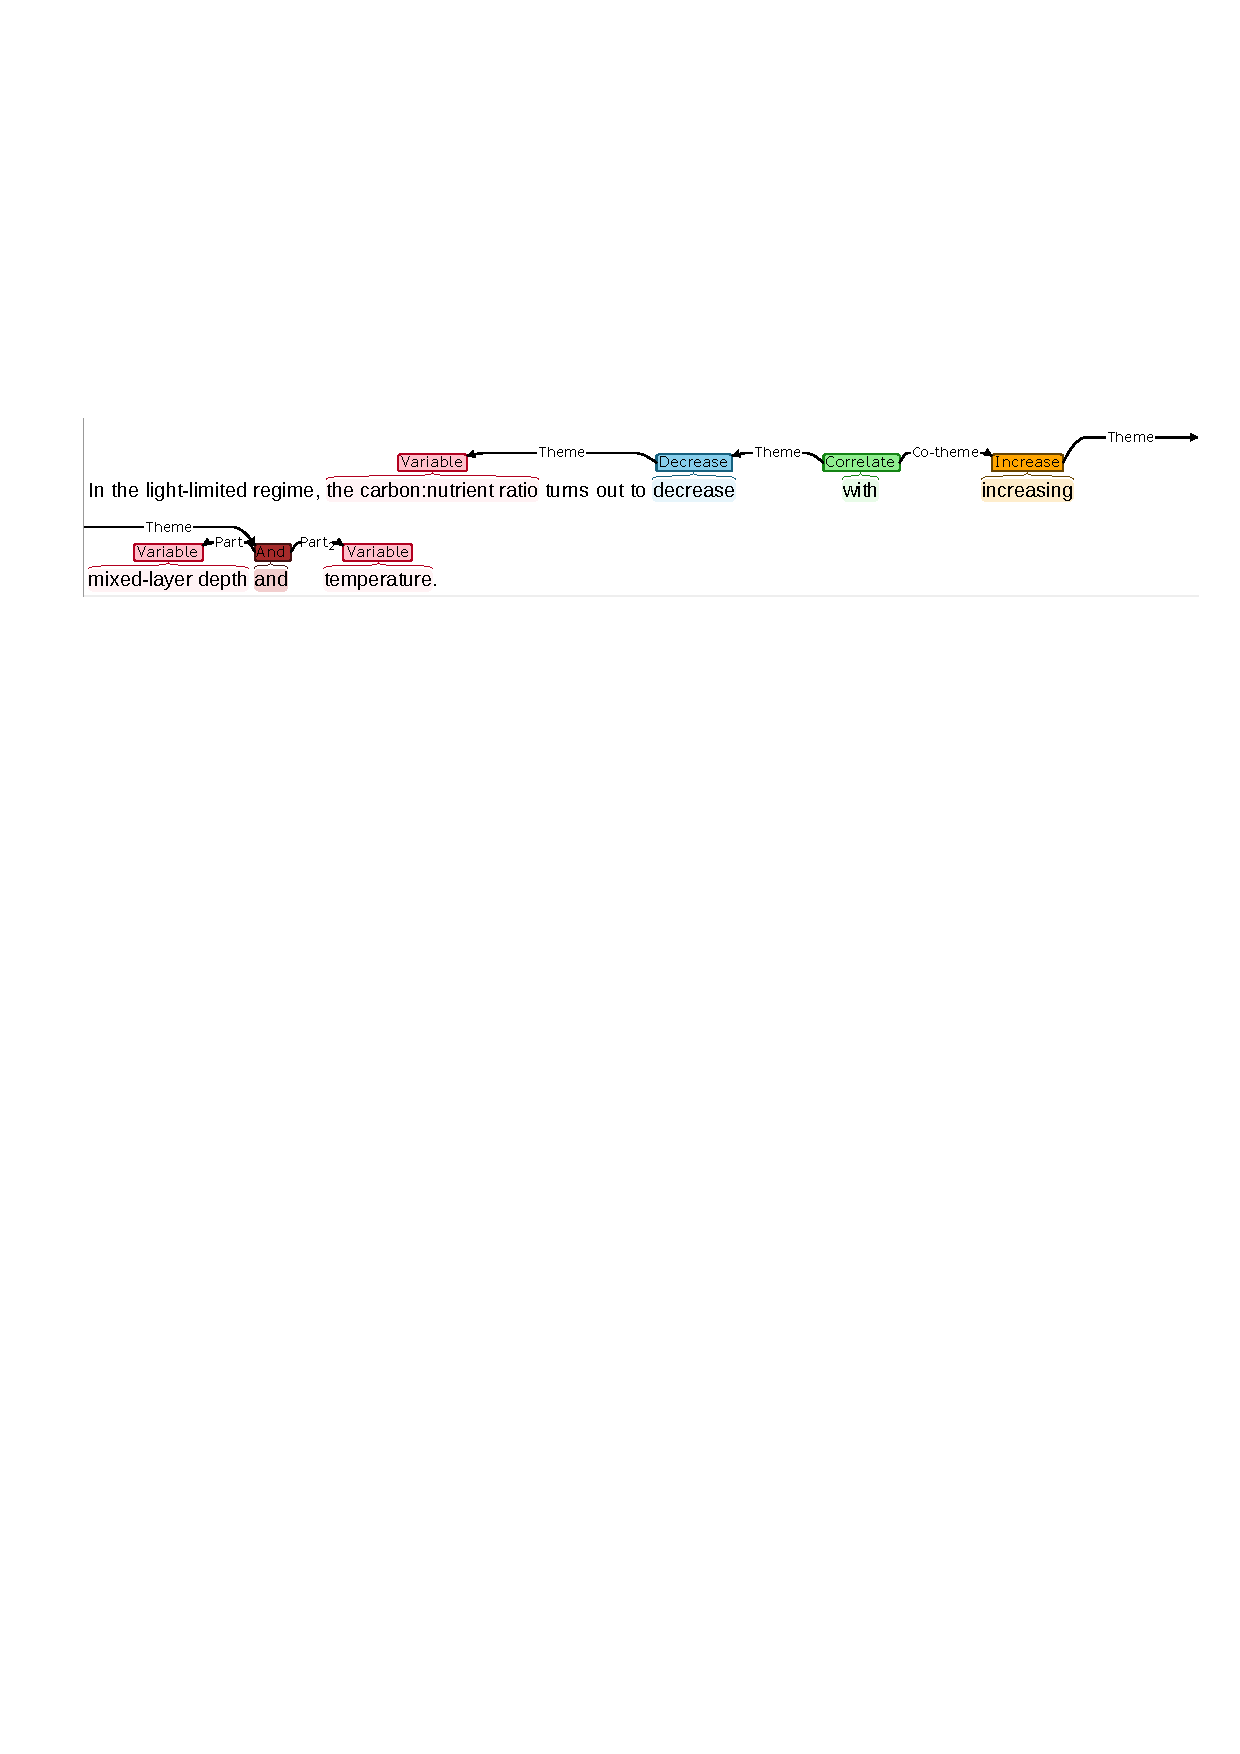
\includegraphics[scale=0.9]{ex2.pdf}}
\framebox[\textwidth]{[ $\uparrow$ mixed-layer depth $\wedge$ $\uparrow$ temperature ]~~~ $\leadsto$~~~$\downarrow$ the carbon:nutrient ratio}
 \caption{Example of a correlation rule extracted from an annotated sentence}
\end{center}
\label{fig:ex2}
\end{figure*}



\begin{figure*}
\begin{center}
\framebox[\textwidth]{
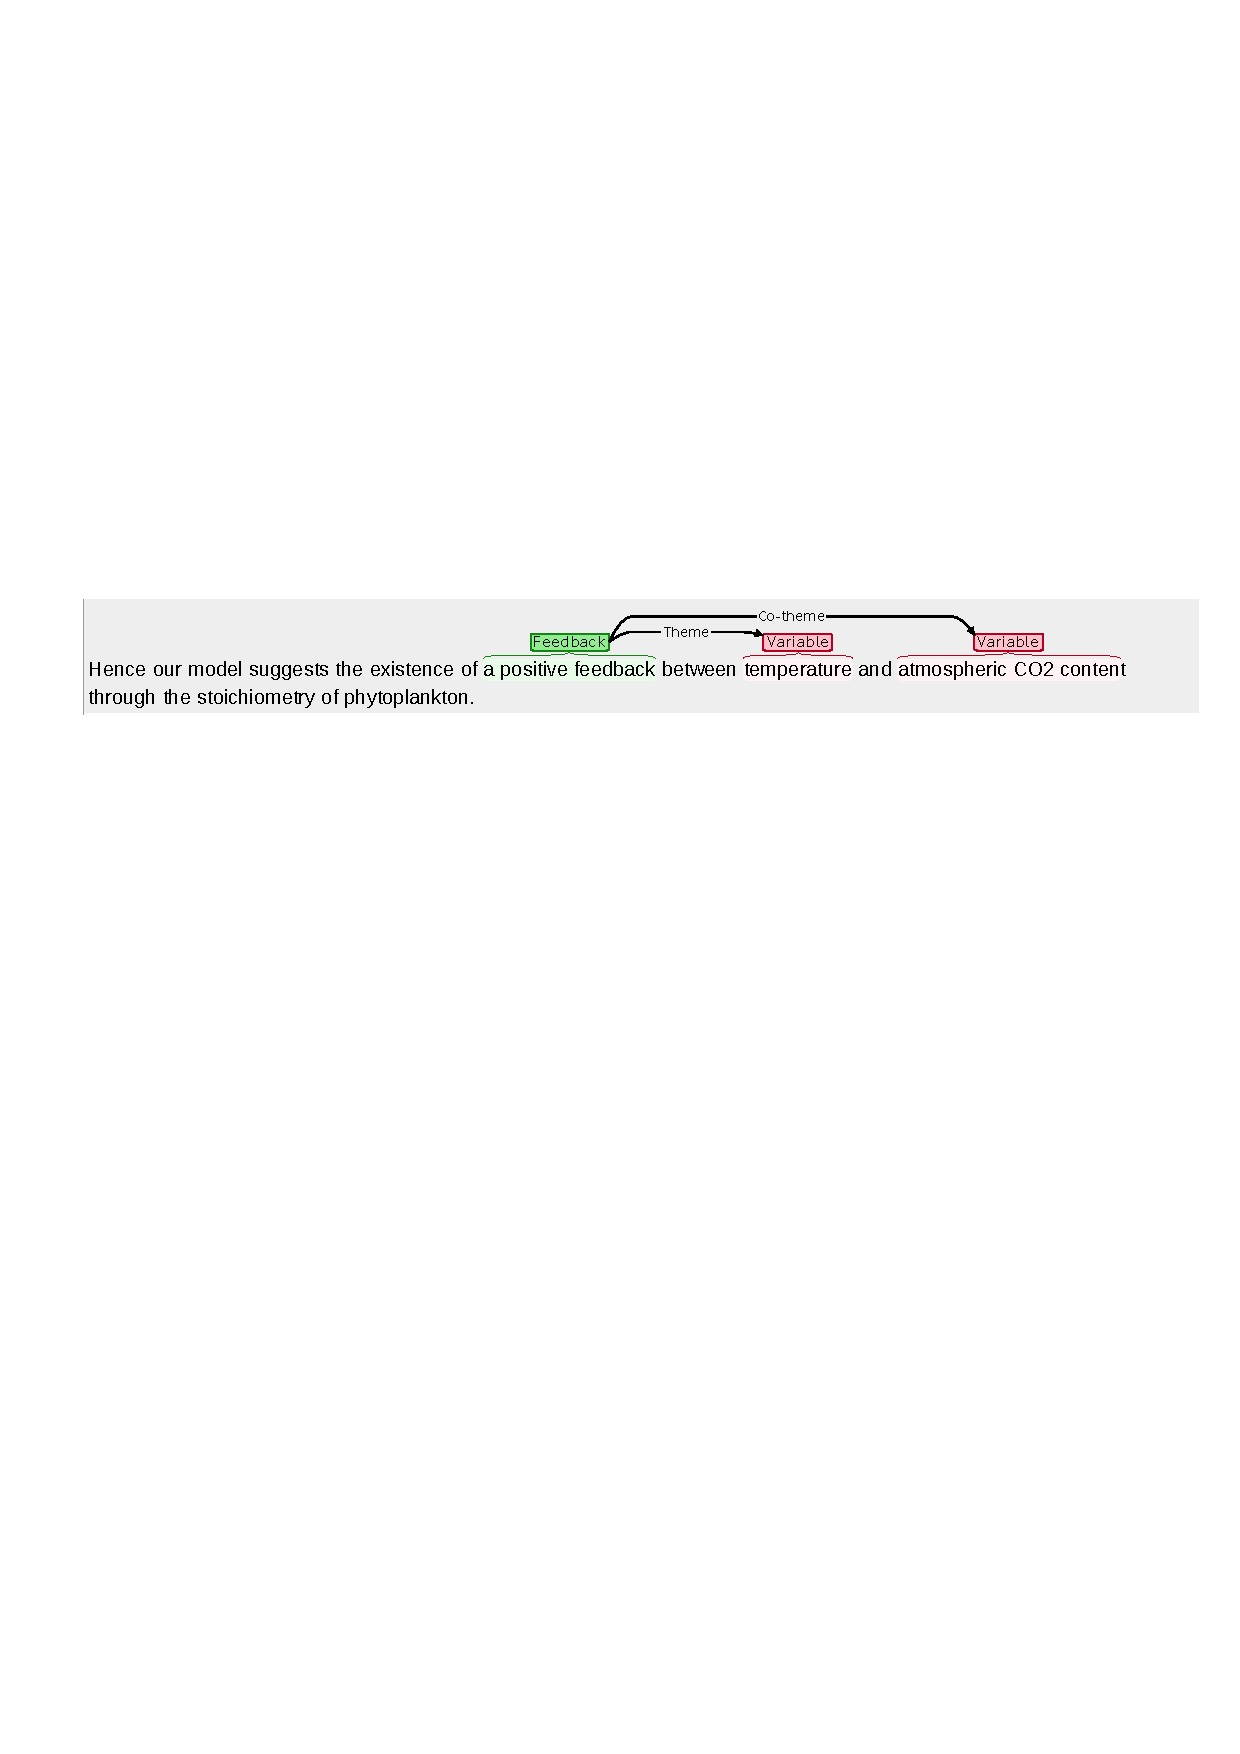
\includegraphics[scale=0.9]{ex3.pdf}}
\framebox[\textwidth]{$\updownarrow$ temperature~~~$\Longleftrightarrow$~~~$\updownarrow$ marine primary production}
 \caption{Example of a feedback rule extracted from an annotated sentence}
\end{center}
\label{fig:ex3}
\end{figure*}


\EM{Proof that it is possible to fully automatically extract intended rule
from proposed annotation.}

%=============================================================================
\section{Discussion}
%=============================================================================
\label{sec:discussion}

\todo[inline]{Automatic annotation:
What aproach do we intend to use?
Generic, unsupervised open IE vs dedicated supervised system?
How well do we think this is going to work?
Bootstrapping and active learning to save annotation costs?
}

\todo[inline]{Variables:
Interpretation of variables in context (anaphora resolution and resolving referring expression);
Linking to ontologies
}
In a cross-disciplinary domain such as Environmental/Climate Science, it is likely that different backgrounds lead to differences in vocabulary\footnote{Here we should put an example of different word usage}.
To Swanson link the statements $A \to B_1$ and $B_2 \to C$, it is necessary to for the system to detect that $B_1 = B_2$ given that $B_1$ and $B_2$ are synonymous.
To this end, it will be necessary to link the annotated variables to concepts in a domain ontology\footnote{Given that we have an ontology, would this be a part of the annotation process, or simply something we do computational later on?}.

\todo[inline]{Reasoning:
How do want to use the extracted rules for reasoning?
Specification/generalization of rules (relation to natural logic?)
How to combine with bckground knowledge?
}
In their NLP-based LBD system, Bitola, \newcite{Hristovski2008NLPinLBD} define certain Discovery Patterns to guide their search through the concept-relation space. A discovery pattern specifies a set of conditions, and a relation that is predicted to hold if the conditions are satisfied. One example from their application is the \emph{Maybe\_treats} pattern, which holds between a drug and a disease if they have an opposite effect on a body function or bodily substance. In the Bitola system the user navigates through the concept-relation chains manually, but it is conceivable to conduct automatic searches for applications of discovery patterns using sub-graph matching.

While potential treatments are of particular interest to the biomedical domain, feedback loops are particularly interesting in the Environmental/Climate Science domain. 
The annotation guidelines presented here have been developed with the goal of facilitating discovery of feedback loop candidates, in the way they focus on quantitative changes in variables rather than plain causal relations\footnote{This sentence should maybe be moved to an earlier stage, as it explains our motivation. Also this is neglecting contradictions/other chains.}.
Feedback loops are normally expressed as a chain of change events where first and last concept are the same, however as there is no theoretical bound to the length of a feedback chain, it is impossible to enumerate the set of all patterns that can give rise to a feedback loop.
Reasoning will therefore follow a production rule inspired approach, where a feedback loop is detected if the system is able to infer a change from a working memory containing only the same change\footnote{Just stating my opinion, I know you might have entirely different conceptions of how the system will work}.


\todo[inline]{Meta-knowledge and context:
Are there examples where context is essential for proper rule application (conditions?)
}

\todo[inline]{User interface:
What kind of use cases do we imagine?
What functionalities (e.g. clicking through to see source text of rule in publication )
What kind of user interface would support this? 
}
The complete system is conceived as a research support system that provides the user with a overview over the relations between the concepts in the domain. 
In the perceived user interface, the user can look up any domain concept.
The user will then be presented with a list of the concepts that are in a relation with the look-up concept. 
By again looking up concepts that are in a relation with the newly selected concept the user can build a chain of related concepts.
The user interface will let the user explore the relation holding between two concepts closely, by providing links to the source sentence(s) from which the relation was extracted. 
Based on the frequency of occurrence of the relation between the two concepts and the source text, the user will the be able to judge the validity of the concept-relation chain.
This should reduce the workload for a researcher by providing easy and comprehensive access to relevant relations in the domain as well as pointers to source texts.

%=============================================================================
\section{Conclusion}
%=============================================================================


\todo[inline]{Conclusions}

%=============================================================================
\section{Acknowledgements}
%=============================================================================

Financial aid from the European Commission (OCEAN-CERTAIN, FP7-ENV-2013-6.1-1; no: 603773) is gratefully acknowledged. 


\section{References}

\bibliographystyle{lrec2006}
\bibliography{biotxtm14}

\end{document}

